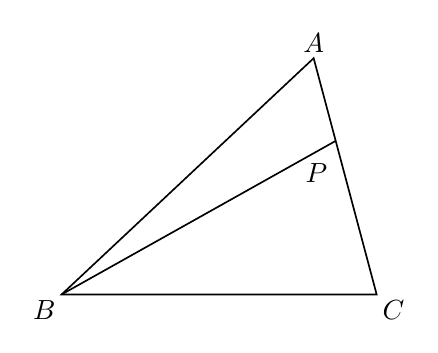
\begin{tikzpicture}[x=1cm,y=1cm,font=\normalsize,
 geometry edge/.style={solid,line width=.6pt},
 geometry mark/.style={solid,line width=.6pt},
 geometry label/.style={font=\normalsize,inner sep=2pt}]
\coordinate (B) at (0,0);
\coordinate (C) at (4,0);
\coordinate (A) at (3.2,3);
\coordinate (P) at (3.48,1.95);
\draw[geometry edge] (B)--(C)--(A)--cycle;
\draw[geometry edge] (B)--(P);
\node[geometry label,above] at (A) {$A$};
\node[geometry label,below left] at (B) {$B$};
\node[geometry label,below right] at (C) {$C$};
\node[geometry label,below,xshift=-7pt,yshift=-6pt] at (P) {$P$};
\end{tikzpicture}
